\section{Method Selection} \label{sec:Clustering}

Clustering with each of the four methods, resulted in tables containing the used settings and a summary of the clustering. The tables are combined based on the exploration method. \autoref{tab:Cluster_Knee} contains the results of the two methods using the Kneedle Algorithm and \autoref{tab:Cluster_DBCV} the results based on using the \gls{DBCV}. Every segment of \gls{IAV} was clustered by each method. By result comparison of methods using $\varepsilon$ exploration by the Kneedle Algorithm (PK and UK) in \autoref{tab:Cluster_Knee}, a major difference in the number of raw clusters stood out. Hybrid \texttt{HDBSCAN} clustering of the only \texttt{PCA} reduced 7-mer vectors resulted in around 60 to 70 raw clusters (\texttt{DBSCAN} part) and 40 to 50 final clusters (standard \texttt{HDBSCAN} part) per segment. The number of final clusters is relative close to the state of the art subtype classification with 18 \gls{HA} and 11 \gls{NA} antibody subtypes \autocite{noauthor_revision_1980}. The UK method results in a way higher number of clusters with no difference of raw and final cluster number. Therefore, the hybrid \texttt{HDBSCAN} clustering only used the \texttt{DBSCAN} part. This can be explained by the overall higher $\varepsilon$ threshold compared to the \texttt{PCA} version (PK). By a higher $\varepsilon$ more points are included in the \texttt{DBSCAN} part of the hybrid clustering. With the \texttt{UMAP} reduction method (UK) in comparison to the one using \texttt{PCA} all vectors of every segment could be clustered with no unclustered vectors. The approach using \texttt{PCA} alone is unable to cluster the vectors of around 10 to 30 sequences per segment. However the number of unclustered for, e.~ g.,~ segment 4 is 6 of 56617 used sequences and, therefore, neglectable $\approx$ 0.01\%. As a comparison, 1191 sequences segment 4 are declared unclassified by the curent subtype convention making $\approx$ 2\%. 

\begin{table}[!hbt]
    \centering
    \caption[Clustering results with the Kneedle Algorithm]{\textbf{Clustering results with the Kneedle Algorithm.} The results of the clustering methods using the Kneedle Algorithm (PK and UK). Listed is every used segment with the number of raw clusters and the final cluster number after hybrid clustering with the given value of $\varepsilon$. The numbers of mixed cluster numbers of H and N denotes number of clusters containing vectors related to more than one subtype. The variance is calculated as the sum of the explained variance by the \texttt{PCA}.}
    \label{tab:Cluster_Knee}
    \pgfplotstableset{
        create on use/method/.style={
            create col/set list={PK, , , , , , , , UK, , , , , , , }
        }
    }
    \pgfplotstablevertcat{\output}{PCA/information.csv}
    \pgfplotstablevertcat{\output}{UMAP/information.csv}
    \pgfplotstabletypeset[
        every nth row={8}{before row=\midrule},
        every head row/.style={
            before row={
                \toprule
                & & \multicolumn{3}{l}{\textbf{\#Cluster}} &  \multicolumn{2}{l}{\textbf{\#Mixed}} & &\\
                \cmidrule(lr){3-5}\cmidrule(lr){6-7}
            },
            after row={
                \midrule
            },
        },
        every last row/.style={
            after row={
                %... & ... & ... & ... & ... & ... & ... & ...\\
                \bottomrule
            },
        },
        begin table=\begin{tabular*}{\textwidth},
        end table=\end{tabular*},
        columns={method,0,1,2,3,5,6,4,7,8},
        columns/method/.style={string type, multicolumn names=l,column name=\textbf{Method}, column type=@{\extracolsep{\fill}\hspace{6pt}}l},
        columns/0/.style={int detect, multicolumn names=l,column name=\textbf{Segment}, column type=r},
        columns/1/.style={int detect, multicolumn names=l,column name=\textbf{Final}, column type=r},
        columns/2/.style={int detect, multicolumn names=l,column name=\textbf{Raw}, column type=r},
        columns/3/.style={multicolumn names=l,column name=\textbf{Normalized}, column type=r},
        columns/4/.style={int detect, multicolumn names=l,column name=\textbf{\#Unclustered}, column type=r},
        columns/5/.style={int detect, multicolumn names=l,column name=\textbf{H}, column type=r},
        columns/6/.style={int detect, multicolumn names=l,column name=\textbf{N}, column type=r},
        columns/7/.style={multicolumn names=l,column name=\textbf{$\varepsilon$}, column type=r},
        columns/8/.style={multicolumn names=l,column name=\textbf{$\text{Var}(X)$}, column type=r},
    ]
    {\output}
\end{table}

Comparing the methods to the ones using the \gls{DBCV} for $\varepsilon$ exploration instead of the Kneedle Algorithm (\autoref{tab:Cluster_DBCV} did not result in much difference for the \texttt{UMAP} reduction with \gls{DBCV} exploration method (UD). The number of clusters found was a little higher compared to the results found with the Kneedle Algorithm exploration. Using \gls{DBCV} to find the optimal $\varepsilon$ with the \texttt{PCA} pipeline (PD) on the other hand changes the results drastically. The number of final clusters was between 9000 and 12000 depending on the segment, with the exception of segment 4. The raw cluster number was equivalent to the total number of sequences for the given segment. Also the number of unclustered sequences was increased by a major amount to around 20\% for some segments, making the method in any case unusable for \gls{IAV} clustering. Only the clustering of segment 4 with \gls{DBCV} $\varepsilon$ exploration (PD) seemed to be as stable as with the Kneedle Algorithm (PK). The number of clusters for the other segments was higher, because the \gls{DBCV} method was searching for the $\varepsilon$ value setting that results in the best \gls{DBCV}. In all the segments except 4 this resulted in a value of zero. Hybrid clustering with a $\varepsilon$ value of zero results in standard \texttt{HDBSCAN} clustering only and is, considering the amount of unclustered sequences, not suited for \gls{IAV} clustering without the hybrid setting. Based on the results in \autoref{tab:Cluster_Knee} and \autoref{tab:Cluster_DBCV}, the best method for \gls{IAV} clustering seemed to be the combination of \texttt{PCA} and the Kneedle Algorithm (PK). It resulted in an appropriate number of clusters and was the only combination using all the benefits of the hybrid \texttt{HDBSCAN} clustering. 

\begin{table}[!hbt]
    \centering
    \caption[Clustering results with the DBCV]{\textbf{Clustering results with the DBCV.} The results of the clustering methods using the \gls{DBCV} (PD and UD). Listed is every used segment with the number of raw clusters and the final cluster number after hybrid clustering with the given value of $\varepsilon$. The numbers of mixed cluster numbers of H and N denotes number of clusters containing vectors related to more than one subtype. The variance is calculated as the sum of the explained variance by the \texttt{PCA}.}
    \label{tab:Cluster_DBCV}
    \pgfplotstableset{
        create on use/method/.style={
            create col/set list={PD, , , , , , , , UD, , , , , , , }
        }
    }
    \pgfplotstablevertcat{\output}{PCA/information_alt.csv}
    \pgfplotstablevertcat{\output}{UMAP/information_alt.csv}
    \pgfplotstabletypeset[
        every nth row={8}{before row=\midrule},
        every head row/.style={
            before row={
                \toprule
                & & \multicolumn{2}{l}{\textbf{\#Cluster}} & \multicolumn{2}{l}{\textbf{\#Mixed}} & & &\\
                \cmidrule(lr){3-4}\cmidrule(lr){5-6}
            },
            after row={
                \midrule
            },
        },
        every last row/.style={
            after row={
                %... & ... & ... & ... & ... & ... & ... & ...\\
                \bottomrule
            },
        },
        begin table=\begin{tabular*}{\textwidth},
        end table=\end{tabular*},
        columns={method,0,1,2,4,5,3,6,7,8},
        columns/method/.style={string type, multicolumn names=l,column name=\textbf{Method}, column type=@{\extracolsep{\fill}\hspace{6pt}}l},
        columns/0/.style={int detect, multicolumn names=l,column name=\textbf{Segment}, column type=r},
        columns/1/.style={int detect, multicolumn names=l,column name=\textbf{Final}, column type=r},
        columns/2/.style={int detect, multicolumn names=l,column name=\textbf{Raw}, column type=r},
        columns/3/.style={int detect, multicolumn names=l,column name=\textbf{\#Unclustered}, column type=r},
        columns/4/.style={int detect, multicolumn names=l,column name=\textbf{H}, column type=r},
        columns/5/.style={int detect, multicolumn names=l,column name=\textbf{N}, column type=r},
        columns/6/.style={multicolumn names=l,column name=\textbf{$\varepsilon$}, column type=r},
        columns/7/.style={multicolumn names=l,column name=\textbf{DBCV}, column type=r},
        columns/8/.style={multicolumn names=l,column name=\textbf{$\text{Var}(X)$}, column type=r},
    ]
    {\output}
\end{table}

To backup this assumption, the results were visualized for better understanding and analysis. Since investigation of all segments would overfill this section, only the methods PK, UK and UD and their clustering behavior on segment 4 were discussed in detail. As described, the \texttt{PCA} method in combination with the \gls{DBCV} (PD) used only standard \texttt{HDBSCAN}, resulting in a very high number of clusters and 20\% unclustered sequences. Therefore, the method is already rejected and not included in the following discussions. Nevertheless, all graphics for the other segments with all used method can be found in the \autoref{chap:Appendix}. 

\begin{figure}[!hbt]
    \centering
    %\begin{adjustbox}{minipage=\dimexpr\textwidth-2\fboxsep-2\fboxrule,fbox}
    \begin{subfigure}[b]{0.475\textwidth}
        \caption[Kneedle Algorithm]{\textbf{Kneedle Algorithm}}
        \label{subfig:PCA_Cluster_Knee_Kneedle_4}            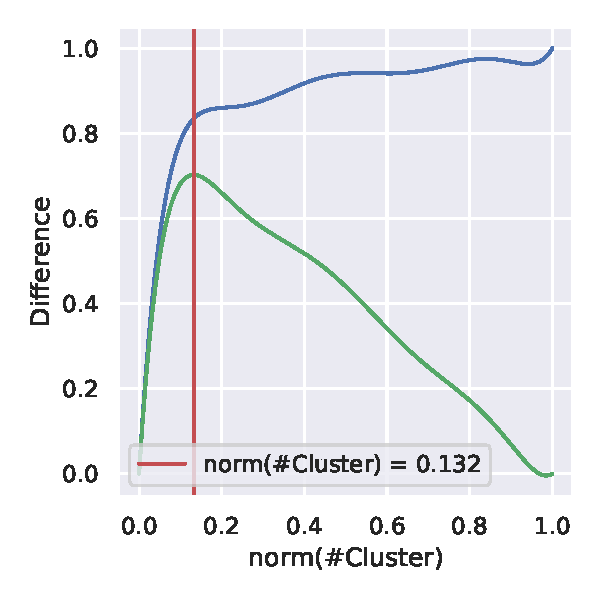
\includegraphics[width=\textwidth]{PCA/Cluster_Knee_Segment_4.pdf}
    \end{subfigure}
    \hfill
    \begin{subfigure}[b]{0.475\textwidth}
        \caption[Kneedle Knee]{\textbf{Kneedle Knee}}
        \label{subfig:PCA_Cluster_Knee_Elbow_4}            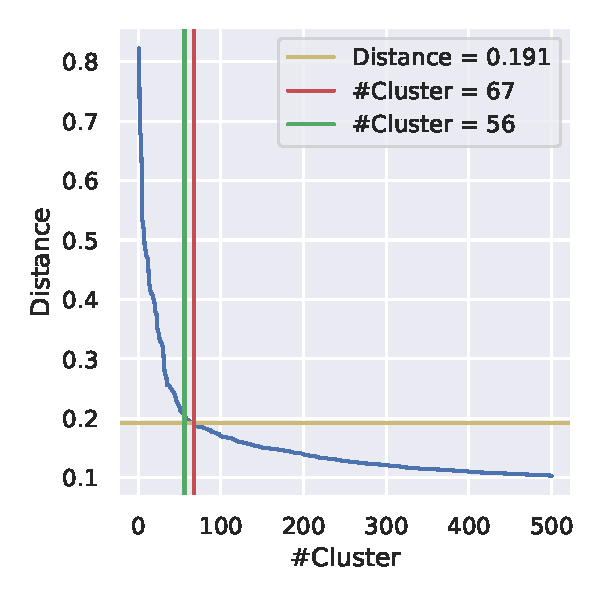
\includegraphics[width=\textwidth]{PCA/Cluster_Elbow_Knee_Segment_4.pdf}
    \end{subfigure}
    \vskip\baselineskip
    \begin{subfigure}[b]{0.475\textwidth}
        \caption[Cluster Distribution]{\textbf{Cluster Distribution}}
        \label{subfig:PCA_Cluster_Knee_Distributione_4}            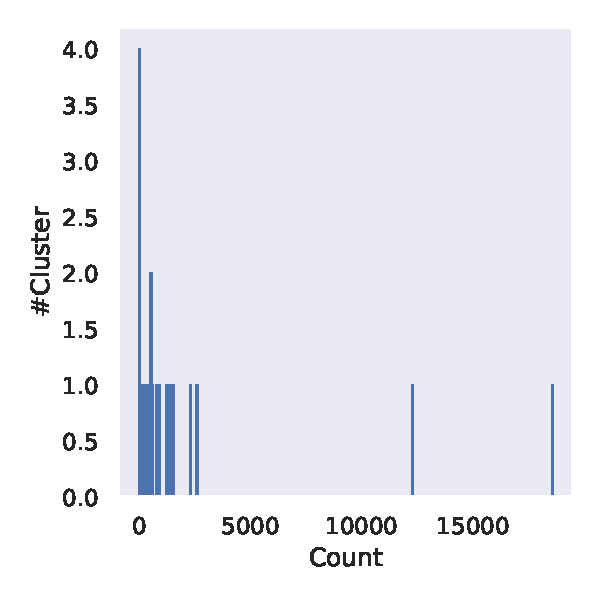
\includegraphics[width=\textwidth]{PCA/Cluster_Distribution_Segment_4.pdf}
    \end{subfigure}
    \hfill
    \begin{subfigure}[b]{0.475\textwidth}
        \caption[Logarithmic Distribution]{\textbf{Logarithmic Distribution}}
        \label{subfig:PCA_Cluster_Knee_Distribution_log_4}            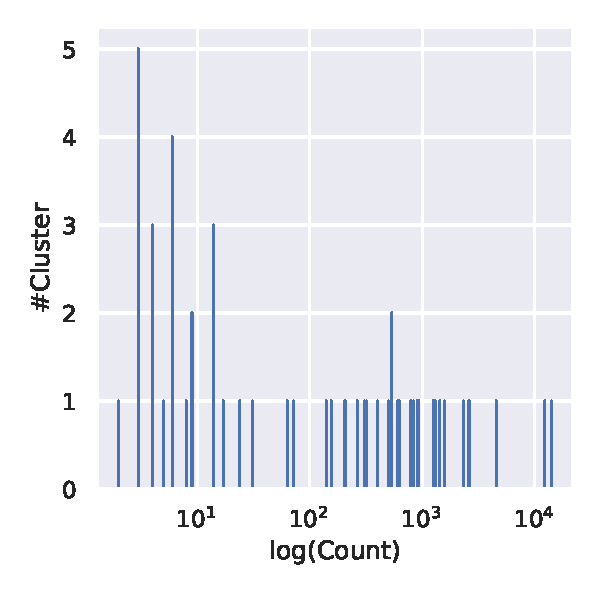
\includegraphics[width=\textwidth]{PCA/Cluster_Distribution_Log_Segment_4.pdf}
    \end{subfigure}
    %\end{adjustbox}
    \caption[Clustering of segment 4 with PK]{\textbf{Clustering of segment 4 with PK.} Segment 4 clustering, using the combination of \texttt{PCA} and the Kneedle Algorithm (PK) results in the given figure. The green curve in the top left sub figure describes the change of the distance in the single linkage tree with increasing normalized cluster number and, therefore, the location of the knee, at the maximum, highlighted by the red line. The blue line is the inverse polynomial representation of the blue line in top right sub figure. The top right sub figure shows the absolute relation of the distance in the single linkage tree to the total number of clusters as the blue line. The red line, indicates the number of raw clusters, by the \texttt{DBSCAN} part of the hybrid \texttt{HDBSCAN} clustering and the final cluster number in green. The yellow line describes the threshold, extracted from the knee and, therefore, the $\varepsilon$ value used to perform the hybrid clustering. The normalized cluster number in the red line in the top left sub figure is equivalent to the raw cluster number in the top right sub figure. The bottom sub figures give information about the distribution of the clusters sizes in continuous and logarithmic scale.}
    \label{fig:PCA_Cluster_Knee_4}
\end{figure}

A big difference in the cluster size distribution stand out, when comparing the method with \texttt{PCA} (PK) to the ones with \texttt{UMAP} (UK and UD). Only the method using \texttt{PCA} and the Kneedle Algorithm created clusters with more than 10000 vectors (\autoref{subfig:PCA_Cluster_Knee_Distributione_4}). The different cluster sizes using \texttt{UMAP} are spreaded more equally with no cluster of 3000 vectors or more (\autoref{subfig:UMAP_Cluster_DBCV_Distribution_4} and \autoref{subfig:UMAP_Cluster_Knee_Distributione_4}). Since the \texttt{UMAP} methods also use prior \texttt{PCA} reduction, the major difference is the additional use of \texttt{UMAP} (\autoref{sec:Dimension_Reduction}). Therefore, the difference in cluster size distribution was most likely caused by \texttt{UMAP}. \texttt{UMAP} not only reduces the dimension of the data but also changes the position of the vectors in the embedded dimension according to the used settings. The \texttt{n\_neighbors=100} setting seems to be most likely the cause of a change of this magnitude. By increasing the number of neighbors the vectors were more crowded in groups to support the bigger picture of the data and, therefore, seemed to build more crowded clusters of equal sizes. 

\vspace{1em}

With the distribution of segment 4 sequences in the data in \autoref{subfig:Frequency_4} in mind, it was expected that a distribution of cluster sizes in segment 4 clustering would in fact approximate the distribution of the sequences in the former one. Therefore, a clustering with \texttt{PCA} in combination with Kneedle Algorithm exploration seemed to give the expected results and appears again as the best method for \gls{IAV} clustering. Taking also the relation of the cluster number and the distance into consideration \autoref{subfig:PCA_Cluster_Knee_Elbow_4} indicated continuous merging of clusters with decreasing cluster number in the linkage tree and easily distinguishable knee point. The behavior is not present in \autoref{subfig:UMAP_Cluster_Knee_Elbow_4} and \autoref{subfig:UMAP_Cluster_DBCV_Elbow_4} in a similar degree.  

% Also the distribution of cluster sizes seems to be more balanced e.~g.~, segment 4 (\autoref{subfig:UMAP_Cluster_Knee_Distributione_4} and \autoref{subfig:UMAP_Cluster_Knee_Distribution_log_4}) than in the \texttt{PCA} approach (\autoref{subfig:PCA_Cluster_Knee_Distributione_4} and \autoref{subfig:PCA_Cluster_Knee_Distribution_log_4}) which could also contribute to the hybrid clustering by \texttt{DBSCAN} alone. With a more distributed number of sequences in the clusters, less very small and very big clusters exist and overall more points are collected in small groups which decreases the chance for single points unaffected by the $\varepsilon$ threshold. 

\vspace{1em}

The results of the method using \texttt{PCA} in combination with the Kneedle Algorithm (PK) were visualized by the cluster tree \autoref{fig:PCA_Clusteree_Knee_4}. Labeling of the tree was performed based on the \gls{HA} antibody subtype as shown in \autoref{subfig:Frequency_4}. Therefore, clusters only containing sequences of a given subtype are labeled as such. If a cluster only contained sequences of one subtype, plus some not classified sequences, the not classified sequences were declared as the subtype too. That way, a clear presentation of the subtype distribution by labeling was possible, since the not classified sequences were very likely to actually belong to an existing subtype when clustered that way. If they actually did not belong to a existing subtype, a cluster only containing these not classified sequences would most likely have occurred, which is not the case. Furthermore, the chance to eventually break the classification of subtypes by declaring not classified sequences to a existing subtype is not given. The clusters are not based on subtypes in any way and the visualization is only for guidance and not possible for any segments other than 4 and 6 anyway. Also, without this assignment of the not classified sequences, no presentation would be possible since they are distributed over mostly all clusters.

\vspace{1em}

If a cluster contains sequences of more than one subtype plus some not classified sequences, no labeling was performed, since the cluster was not homogeneous for one subtype and a declaration of the unclassified was not possible. In the following the term vector is mostly replaced by sequence to aid the discussion in terms of tree placement and subtype relation. Since the vectors represent the sequences, the terms are linked to each other and used as synonyms. %Exceptions are alignments that did not involve the vector representations, only the sequences. 

\begin{table}[!hbt]
    \centering
    \caption[Unclassified sequences in segment 4 cluster 29 with PK]{\textbf{Unclassified sequences in segment 4 cluster 29 with PK.} The \glspl{MSA} mean distance of the given sequences in comparison to a sample of H9 sequences of the same cluster and a sample of unclassified sequences present in other clusters. Only the first 20 columns are presented here, the full table can be found in the projects GitHub Repository\footnotemark.}
    \label{tab:PCA_Error_4_29}
    \pgfplotstabletypeset[
        every head row/.style={
            before row={
                \toprule
            },
            after row={
                \midrule
            },
        },
        every last row/.style={
            after row={
                ... & ... & ... \\
                \bottomrule
            },
        },
        begin table=\begin{tabular*}{0.75\textwidth},
        end table=\end{tabular*},
        columns={0,1,2},
        columns/0/.style={string type,multicolumn names=l,column name=\textbf{Accession}, column type=@{\extracolsep{\fill}\hspace{6pt}}l},
        columns/1/.style={multicolumn names=l,column name=\textbf{H9}, column type=l},
        columns/2/.style={multicolumn names=l,column name=\textbf{unclassified}, column type=l},
    ]
    {PCA/error_segment_4_cluster_29_difference_head.csv}
\end{table}

The prime example of the not classified sequence annotation is the yellow colored cluster 29 of subtype H9 (\autoref{fig:PCA_Clusteree_Knee_4} \textbf{\textsf{A}}). While the vectors of all sequences of subtype H9 are accumulated in this single cluster, the cluster size of 1569 is bigger than the number of H9 sequences in \autoref{subfig:Frequency_4} with 1454. This is justified by the presence of 115 not classified sequences in the cluster which are declared as H9, since only H9 and unclassified sequences are present in the cluster. The declaration of the unclassified sequences to be the H9 sequences is supported by the very small evolutionary distance values for the unclassified sequences in comparison to a sample of H9 sequences from the same cluster (\autoref{tab:PCA_Error_4_29}). The sequences were also compared to unclassified sequences from other clusters to prove the smaller evolutionary distance to H9 sequences. This comparison was performed to prove that, even when only used for visualization reasons, the annotation of not classified sequences in that way is most likely true.

\vspace{1em}

The number of clusters for a given subtype of \gls{HA} antibody seems to correspond roughly to the overview of sequences in \autoref{subfig:Frequency_4}. Clusters of very low represented subtypes, like H15, contain mostly all the subtypes sequences, while the high represented subtypes sequences, like H1 and H3, are spreaded over more clusters.

\begin{figure}[!hbt]
    \centering
    \footnotesize
    \begin{tikzpicture}
        \node[anchor=south west,inner sep=0] (image) at (0,0) {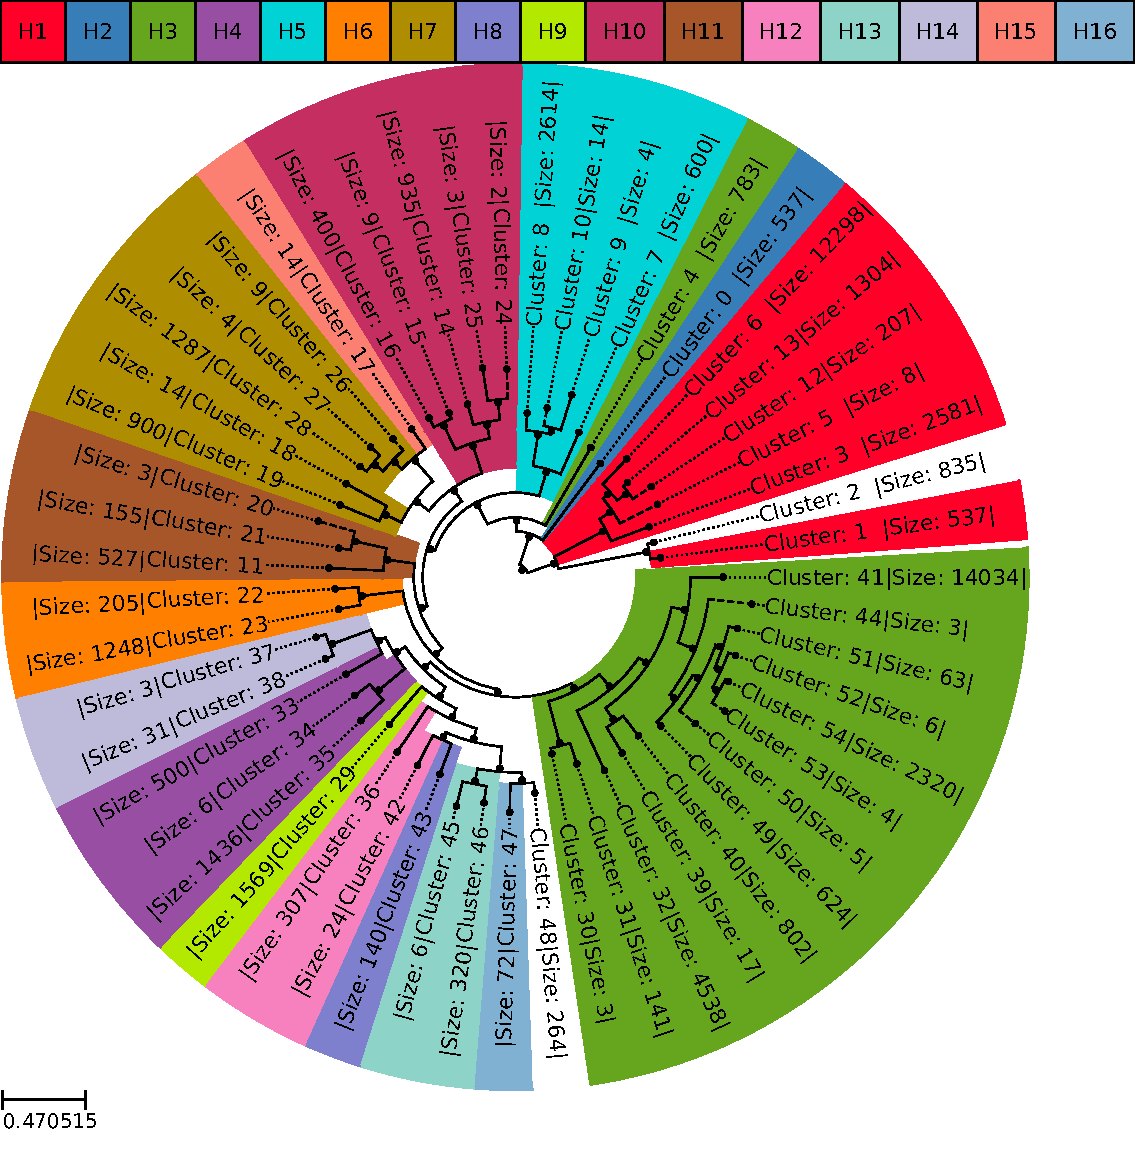
\includegraphics[width=\textwidth]{PCA/Clustertree_Segment_4_H_Knee.pdf}};
        \begin{scope}[x={(image.south east)},y={(image.north west)}]
            %\draw[help lines,xstep=.1,ystep=.1] (0,0) grid (1,1);
            \node at (0.16,0.18) [arrowstyle=1.0cm, arrowfillR, anchor=east, rotate=45] {\textbf{\textsf{A}}};
            \node at (0.5,0.08) [arrowstyle=1.0cm, arrowfillR, anchor=east, rotate=45] {\textbf{\textsf{B}}};
            \node at (0.89,0.62) [arrowstyle=1.0cm, arrowfillR, anchor=east, rotate=180] {\rotatebox{180}{\textbf{\textsf{C}}}};
            \node at (0.7,0.9) [arrowstyle=1.0cm, arrowfillR, anchor=east, rotate=180] {\rotatebox{180}{\textbf{\textsf{D}}}};
        \end{scope}
    \end{tikzpicture}

    \caption[Clustering tree of segment 4 with PK]{\textbf{Clustering tree of segment 4 with PK.} The cluster tree of segment 4 clustering, using the combination of \texttt{PCA} and the Kneedle Algorithm (PK) (\autoref{fig:PCA_Cluster_Knee_4}). The labeling of the clusters in the tree is based on the subtype of the contained sequences. Unclassified sequences of a cluster are reclassified as a given subtype if sequences of only this subtype are present in the cluster in addition to the unclassified ones. Unlabeled clusters contain sequences from at least two subtypes and zero or more unclassified sequences. Two clusters are mixed since containing sequences of more than one subtype (\autoref{tab:Cluster_Knee}). These non homogeneous clusters are marked by \textbf{\textsf{B}} and \textbf{\textsf{C}}. The cluster 29 marked by \textbf{\textsf{A}} is an example for an cluster consisting of all sequences from a given subtype. The misplaced cluster from subtype H3 is marked by \textbf{\textsf{D}}. Dotted lines in the tree indicate the same host.}
    \label{fig:PCA_Clusteree_Knee_4}
\end{figure}

Striking anomalies divergent from the expected nearly uniform allocation of the subtypes in \autoref{fig:PCA_Cluster_Knee_4} are noted by \textbf{\textsf{B}}, \textbf{\textsf{C}} and \textbf{\textsf{D}} and are discussed in the following. For final acceptance of the method PK as the prime \gls{IAV} clustering method proposed in this project, the cluster tree was compared to a similar one created on the results from method UK (\autoref{fig:UMAP_Clusteree_Knee_4}. While the labeling of the cluster tree of method PK resemble the subtype classification of \gls{IAV} very closely, no recognizable subtype separation is present in the cluster tree of UK. 
\footnotetext{\url{https://github.com/ahenoch/Masterthesis.git}}